\documentclass[11pt,aspectratio=169]{beamer}
%%%%%%%%% GENERAL PACKAGES
%\usepackage[dvipsnames]{xcolor}
%\usepackage{pdfpages}
%\usetheme[progressbar=frametitle]{metropolis}
%\setbeamercolor{background canvas}{bg=white}
%\usepackage{appendixnumberbeamer}
%\usepackage{booktabs}
%\usepackage[scale=2]{ccicons}
%\usepackage{pgfplots}
%\usepgfplotslibrary{dateplot}
%\usepackage{xspace}
%\newcommand{\themename}{\textbf{\textsc{metropolis}}\xspace}
%\usepackage[absolute,overlay]{textpos}






%%%%%%%%% COLOR THEME

% Define some colors:
\definecolor{DarkFern}{HTML}{407428}
\definecolor{DarkCharcoal}{HTML}{4D4944}
\definecolor{AlertColor}{RGB}{89,124,158}
\definecolor{HighLight}{RGB}{96,95,134}
\definecolor{Important}{RGB}{234,122,133}
\definecolor{Yellow}{HTML}{00539C}
\colorlet{Fern}{DarkFern!85!white}
\colorlet{Charcoal}{DarkCharcoal!85!white}
\colorlet{LightCharcoal}{Charcoal!50!white}
\colorlet{HighLight2}{AlertColor}
\colorlet{DarkRed}{red!70!black}
\colorlet{DarkBlue}{blue!70!black}
\colorlet{DarkGreen}{green!70!black}
\definecolor{RoyalBlue}{HTML}{00539C}
\definecolor{Peach}{HTML}{EEA47F}
\definecolor{ForestGreen}{HTML}{2C5F2D}
\definecolor{MossGreen}{HTML}{E8FCC9}
\definecolor{SeaGreen}{HTML}{2E8B57}
% Use the colors:
\setbeamercolor{title}{fg=Fern}
\setbeamercolor{frametitle}{fg=MossGreen,bg=ForestGreen}
\setbeamercolor{normal text}{fg=Charcoal!70!black}
\setbeamercolor{block title}{fg=black,bg=Fern!25!white}
\setbeamercolor{block body}{fg=black,bg=Fern!10!white}
\setbeamercolor{block title alerted}{fg=black,bg=DarkRed!25!white}
\setbeamercolor{block body alerted}{fg=black,bg=DarkRed!10!white}
\setbeamercolor{alerted text}{fg=DarkRed}
\setbeamercolor{itemize item}{fg=Charcoal}



%%%%%%%%% OTHER COMMANDS
\newcommand{\indep}{\perp\!\!\! \perp}
\newcommand{\comment}[1]{}
\newcommand{\bs}{\boldsymbol}
\newcommand{\tr}{\text{trace}}
\newcommand{\sgn}{{\rm sgn}}
\def\T{\top}
%\newcommand{\det}{\text{det}}
\newcommand{\var}{\mathrm{var}}
\newcommand{\cC}{{\cal C}}
\renewcommand{\d}{{\rm d}}
\newcommand{\cG}{{\cal G}}
\newcommand{\cV}{{\cal V}}
\newcommand{\cE}{{\cal E}}
\newcommand{\cM}{{\cal M}}
\newcommand{\cP}{{\cal P}}
\newcommand{\cX}{{\cal X}}
\newcommand{\cY}{{\cal Y}}
\newcommand{\X}{\mathbf{X}}
\newcommand{\Y}{\mathbf{Y}}
\newcommand{\x}{\mathbf{x}}
\newcommand{\y}{\mathbf{y}}
\newcommand{\z}{\mathbf{z}}

\newcommand{\argmin}{\operatornamewithlimits{argmin}}
\newcommand{\eps}{\varepsilon}
\newcommand{\<}{\langle}
\renewcommand{\>}{\rangle}


%

\setbeamertemplate{navigation symbols}{}
\setbeamertemplate{footline}[text line]{%
    \hfill\strut{%
        \scriptsize\sf\color{black!60}%
        \quad\insertframenumber/\inserttotalframenumber
    }
    %\hfill
    }


\usenavigationsymbolstemplate{}
\setbeamersize{text margin left=.2cm,text margin right=.2cm} 
\addtobeamertemplate{frametitle}{}{\vspace{-1.2mm}}
\setbeamertemplate{itemize item}{$\bullet$}

\setbeamertemplate{itemize subitem}{\tiny\raise1.5pt\hbox{\donotcoloroutermaths$\blacktriangleright$}}
\setbeamertemplate{itemize subsubitem}{\tiny\raise1.5pt\hbox{\donotcoloroutermaths$\blacktriangleright$}}
\setbeamertemplate{enumerate item}{\insertenumlabel.}
\setbeamertemplate{enumerate subitem}{\insertenumlabel.\insertsubenumlabel}
\setbeamertemplate{enumerate subsubitem}{\insertenumlabel.\insertsubenumlabel.\insertsubsubenumlabel}
\setbeamertemplate{enumerate mini template}{\insertenumlabel}






\newcommand{\TODO}[1]{{\color{red}{[TODO: #1]}}}


\newcommand{\R}{\mathbb R}
\newcommand{\E}{\mathbb E}
\renewcommand{\P}{\mathbb P}


\DeclareMathOperator*{\cov}{cov}


\newsavebox{\zerobox}
\newenvironment{nospace}
{\par\edef\theprevdepth{\the\prevdepth}\nointerlineskip
  \setbox\zerobox=\vtop to 0pt\bgroup
  \hrule height0pt\kern\dimexpr\baselineskip-\topskip\relax
}
{\par\vss\egroup\ht\zerobox=0pt \wd\zerobox=0pt \dp\zerobox=0pt
  \box\zerobox}

\usepackage{soul}
\makeatletter
\let\HL\hl
\renewcommand\hl{%
  \let\set@color\beamerorig@set@color
  \let\reset@color\beamerorig@reset@color
  \HL}
  \makeatother

\usepackage{tikz}

%\usecolortheme{whale}

\title[Calculus and Linear Algebra]{Lecture 1 : Calculus}
\author[Piotr Zwiernik, Barcelona School of Economics]{Piotr Zwiernik \\ $\;$\\
Mathematics Brush-up\\ $\;$\\ $\;$\\

\includegraphics[width=1in]{img/bse.png}  
}
\date{}

%\beamerdefaultoverlayspecification{<+->}

\begin{document}
\begin{frame}
\titlepage
\end{frame}



%--------------- slide 2  ----------------%


%--------------- slide 1  ----------------%
\begin{frame}{Goal of the course}

\textcolor{SeaGreen}{Review} core tools of calculus that power modern economics, finance, and data-driven policy.\\[6mm]

These tools are \textcolor{SeaGreen}{crucial} in courses on micro/macro, econometrics, finance, and machine learning.\\[6mm]

\textcolor{SeaGreen}{Warm up} before the Master starts: sharpen intuition, not just technique.\\[6mm]

\textcolor{SeaGreen}{Main references:} 
\begin{enumerate}
\item {\it Mathematics for Economists} by C. P. Simon and L. Blume
\item {\it Mathematics of Economics and Business} by F. Werner and Y. N. Sotskov
\end{enumerate}
\end{frame}

\begin{frame}{Cultivate a Critical Mindset}
Technical knowledge requires effort. 
\begin{itemize}
  \item[$\bullet$] \textbf{If a step feels ``magical'', stop.} Ask \emph{why} it works, not just \emph{how}.\\[3mm]
  \item[$\bullet$] \textbf{Challenge every answer --- especially given by LLMs.}\\
        Large-language models can sound confident yet be wrong; verify with first principles or a textbook.\\[3mm]
  \item[$\bullet$] \textbf{Use multiple lenses.}\\  
        Check special cases, sketch a graph, test numerically, or search for a counterexample.
\end{itemize}
\end{frame}


\begin{frame}{Index}

\begin{enumerate}
\item Sequences and series
\item Functions of one variable
\item Differentiation
\item Integration
\item Vectors
\item Matrices and determinants
\item Systems of linear equations
\item Eigenvalue problems and quadratic forms
\item Functions of several variables
\item Introduction to differential equations
\end{enumerate}
\end{frame}


\begin{frame}{Sequences }
%
A \textcolor{SeaGreen}{sequence} is an ordered list of real numbers $(a_1,a_2,\ldots)$ indexed by $n\in\mathbb{N}$. \\[3mm]

\textcolor{SeaGreen}{Notation:} $\{a_n\}_{n=1}^{\infty}$ where each $a_n\in\mathbb{R}$.\\[6pt]
Define by a \textcolor{SeaGreen}{formula} or a \textcolor{SeaGreen}{recursion}.
\vskip 10pt
\textcolor{SeaGreen}{Examples:} 
\begin{enumerate}
\item $a_n=\dfrac{n-1}{2n+1}$\quad  \begin{tiny}$(a_1=0, a_2=\frac15,a_3=\frac27,\ldots)$ \end{tiny}
\item $a_1=2, \; a_{n+1}=2a_n-1$\quad  \begin{tiny}$(2,3,5,9,\ldots)$ \end{tiny}
\item $a_1=1, a_2=1, \; a_{n+1}=a_n+a_{n-1}$\quad  \begin{tiny}(Fibonacci)\end{tiny}
\item \alert{Arithmetic}: $a_{n}=a_1+(n-1)d$
\item \alert{Geometric}: $a_n=a_1 r^{\,n-1}$
\end{enumerate}
%
\end{frame}

\begin{frame}{Why sequences show up in modern econ/data}
%
\textcolor{SeaGreen}{Where they appear:}
\begin{itemize}
\item \textbf{User metrics:} daily active users (DAU) over days $n$.\\[3mm]
\item \textbf{Inflation tracking:} monthly CPI/CPIH index $a_n$.\\[3mm]
\item \textbf{Training loss:} $a_n$ = loss after $n$ gradient steps (decreasing sequence).\\[3mm]
\item \textbf{Carbon budgets:} remaining allowance after $n$ years.\\[6mm]
\end{itemize}
\textcolor{SeaGreen}{Read} Ch. 2 Werner-Sotskov.\quad
\textcolor{SeaGreen}{Exercises:} 2.4, 2.5, 2.7 (Werner-Sotskov)
%
\end{frame}



\begin{frame}{Small motivating examples}
\begin{enumerate}
\item \textbf{EAR vs APR in FinTech.}  
Let \( P \) be the initial investment. If a platform advertises an \textit{annual percentage rate} (APR) \( R \) but compounds \( m \) times/year, then after \( n \) years:
\[
a_n = P\left(1+\frac{R}{m}\right)^{mn}.
\]
The one-year \textit{effective annual rate} (EAR) is:
\[
\left(1+\frac{R}{m}\right)^m - 1.
\]
{\small (APR is the quoted yearly rate without compounding; APY/EAR accounts for compounding.)}\\[3mm]

%\item \textbf{Subscription growth.}  
%If a product grows at a net rate \( r \) per period (after accounting for cancellations, called “churn”), then:
%\[
%\text{Subs}_{n} = \text{Subs}_{0}(1+r)^n.
%\]

\item \textbf{Creator economy revenue.}  
If the number of views per video is \( v_n \) and the cost-per-thousand views (\textit{CPM}) is \( c \),  
total revenue over \( n \) videos is:
\[
s_n = \sum_{k=1}^n c\,v_k.
\]
\end{enumerate}
\end{frame}

\begin{frame}{Properties of a sequence}

A sequence is \textcolor{SeaGreen}{increasing} if $a_{n+1}\ge a_n$ (strictly if $>$).\\[3mm]
\textcolor{SeaGreen}{Decreasing} if $a_{n+1}\le a_n$ (strictly if $<$).\\[3mm]
\textcolor{SeaGreen}{Monotone} if increasing or decreasing.\\[3mm]
\textcolor{SeaGreen}{Bounded} if $\exists C>0$ s.t. $|a_n|\le C$ for all $n$.\\[5mm]
\vskip 8pt
\textcolor{SeaGreen}{Examples:} 
\begin{enumerate}
\item $a_n=2(n-1)^2-n$ is strictly increasing \begin{tiny}(since $a_{n+1}-a_n=4n-3>0$)\end{tiny}
\item $a_n=1/n^2$ is bounded \begin{tiny}($0<a_n\le 1$)\end{tiny}
\item \textbf{Training loss:} if a learning rate is sensible, $a_n=$loss often decreases and is bounded below by $0$ $\Rightarrow$ convergent in many practical cases.
\end{enumerate}
\end{frame}

{
\begin{frame}[plain]
\centering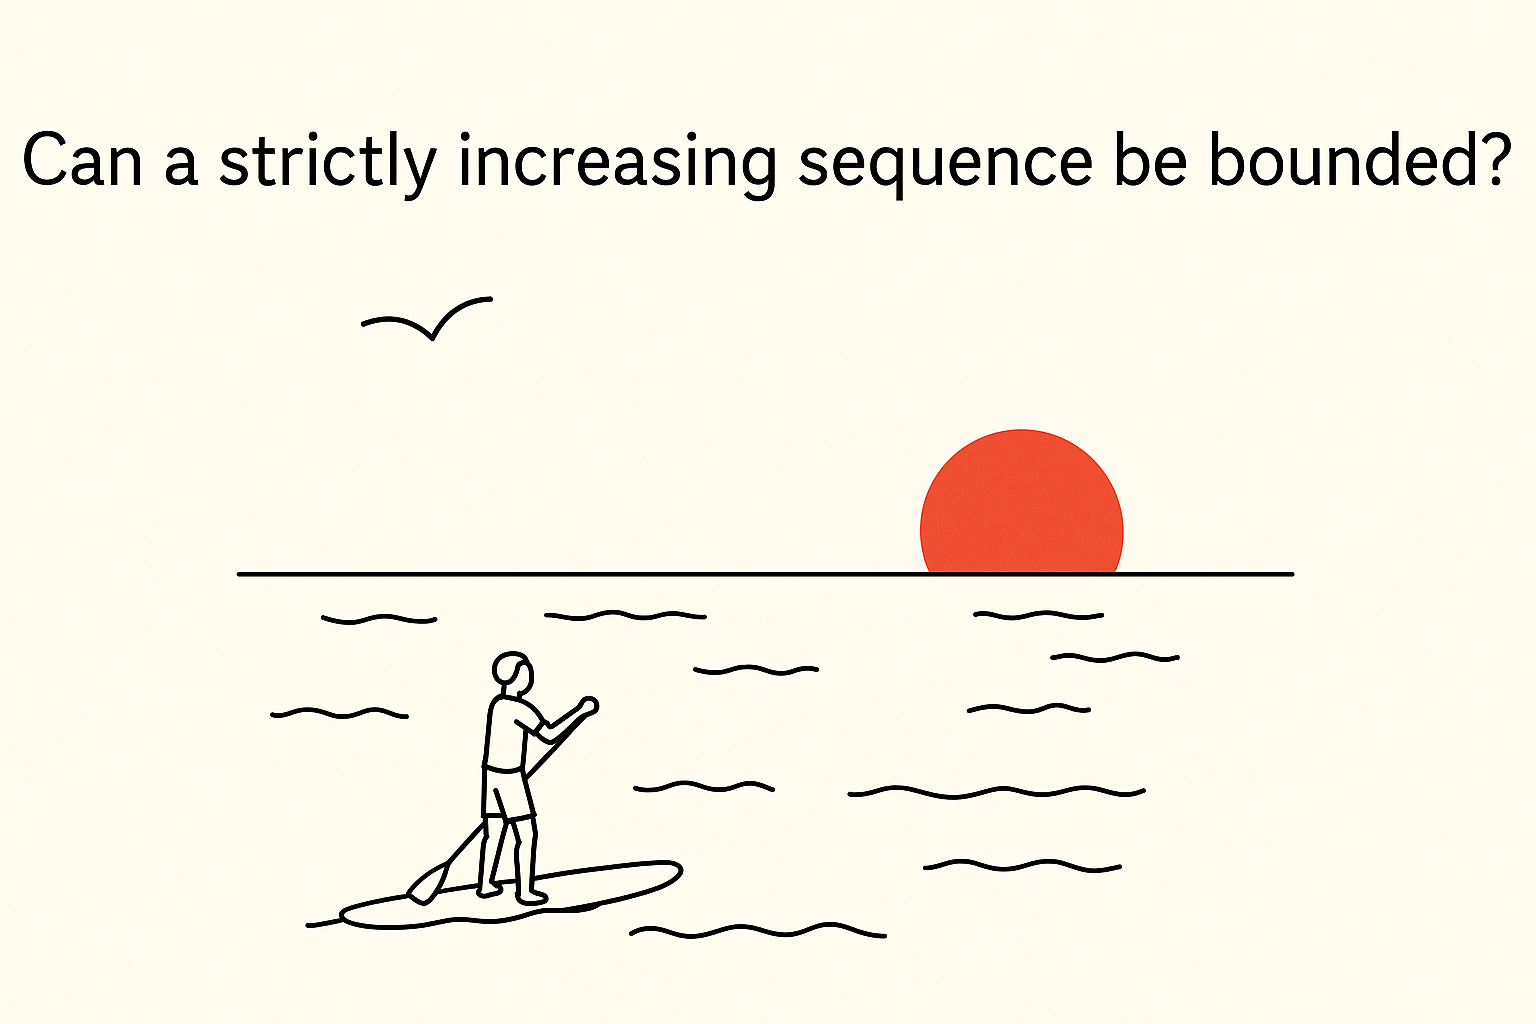
\includegraphics[scale=0.27]{vbreaks/question1.png}
\end{frame}
}


\begin{frame}{Limit of a sequence}
 A real number $a$ is the \alert{limit} of $\{a_n\}$ if as $n\to\infty$, $a_n$ gets arbitrarily close to $a$. \textcolor{SeaGreen}{Notation:} \hl{$\lim_{n \rightarrow \infty} a_n=a$}.
\vskip 8pt
A sequence is \textcolor{SeaGreen}{convergent} if it has a limit; otherwise it \textcolor{SeaGreen}{diverges}.
\vskip 8pt
\textcolor{SeaGreen}{Examples} 
\begin{enumerate}
\item $a_n=\frac{1}{n^2}\to 0$
\item $a_n=(-1)^n$ has no limit
\item $a_n=n^2\to \infty$
\item $a_n=r^n\to 0$ if $|r|<1$; diverges if $r>1$; no limit if $r\le -1$.
\end{enumerate}
\end{frame}



\begin{frame}{Epsilon-definition}
\begin{alertblock}{Definition: $a=\lim_{n\to\infty}a_n$}
\qquad$
\forall \epsilon >0 \quad\exists N_\epsilon\quad\text{s.t.}\;\;\forall n>N_\epsilon:\qquad |a_n-a| < \epsilon.
$	
\end{alertblock}

 \textcolor{SeaGreen}{Example:}  $a_n=\dfrac{1}{n}\to 0$. For any $\epsilon>0$, take $N_\epsilon>\frac{1}{\epsilon}$. \\[4mm]
 \textcolor{SeaGreen}{Checks:} 
 \begin{itemize}
 	\item $\lim a_n=a$ if and only if $\lim |a_n-a|=0$.
 	\item If $a_n=a$ for all $n$, then $\lim a_n=a$.
 \end{itemize}
\bigskip
\begin{block}{If formal definition hard to work with, try to squeezing with easier bounds}
If $0<\frac{1}{2n^2-1}\le \frac{1}{n}$ for $n\ge 1$, then $\lim \frac{1}{2n^2-1}=0$.
\end{block}
\end{frame}

\begin{frame}{Limits that matter in practice}

\textcolor{SeaGreen}{Classics} 
\begin{enumerate}
\item $\Bigl(1+\frac{1}{n}\Bigr)^n \to e$
\item $\Bigl(1+\frac{x}{n}\Bigr)^n \to e^{x}$ for any real $x$
\end{enumerate}

\textcolor{SeaGreen}{Continuous compounding \& APY:} if APR is $R$, then
\[
\lim_{m\to\infty}\Bigl(1+\frac{R}{m}\Bigr)^m=e^R,\quad
\text{EAR}=e^R-1.
\]
\textcolor{SeaGreen}{Example:} APR $=8\%$ $\Rightarrow$ EAR $\approx 8.329\%$.
\end{frame}

\begin{frame}{Monotone convergence and algebra of limits}
\begin{alertblock}{Theorem}
Every bounded monotone sequence is convergent.	
\end{alertblock}
{\small (Just bounded or just monotone is not enough in general) }\\[3mm]
\textcolor{SeaGreen}{Example:} the sequence $a_1=1, \; a_{n+1}=\sqrt{3a_n}$ is bounded by $3$ \begin{tiny} (proof by induction) \end{tiny} and strictly increasing \begin{tiny} (since $\frac{a_{n+1}}{a_n}>1$)\end{tiny}, thus convergent.\\[3mm]
\begin{block}{Algebra of limits}
If $\lim a_n=a$ and $\lim b_n=b$, then
\[
\lim (a_n+b_n)=a+b,\quad 
\lim (a_n b_n)=ab,\quad 
\lim \frac{a_n}{b_n}=\frac{a}{b} \;\text{ if }b_n,b\neq 0.
\]	
\end{block}
%\smallskip
%\textcolor{SeaGreen}{Data view:} A smoothed KPI (moving average) can converge even when the raw series is noisy, if underlying trend is stable and bounded perturbations vanish.
\end{frame}



\begin{frame}{Partial sums and series}
The \textcolor{SeaGreen}{nth partial sum} $s_n$ of $\{a_n\}$ is
\[
s_n=\sum_{k=1}^n a_k.
\]
\textcolor{SeaGreen}{Examples} 
\begin{enumerate}
\item Arithmetic sequence $a_n=a_1+(n-1)d$:\;\;\; $s_n=n a_1+\dfrac{n(n-1)}{2}d$
\item Geometric sequence $a_n=a_1 r^{n-1}$, $r\neq 1$:\;\;\; $s_n=a_1 \dfrac{1-r^n}{1-r}$
\end{enumerate}
\medskip
\textcolor{SeaGreen}{Use-cases:}
\begin{itemize}
\item Let \emph{margin} be the profit earned per customer per period and $p$ be the customer retention rate. The total profit from a single customer over \( n \) periods is: \hl{$s_n = \sum_{k=1}^n \text{margin} \cdot p^k$}.

\item  Let \( E_k \) be the emissions produced in period \( k \) (e.g., in tonnes of CO\(_2\)).  
Then the total emissions over \( n \) periods are: \hl{$s_n = \sum_{k=1}^n E_k$}, which can be compared to a fixed carbon budget.
\end{itemize}
\end{frame}

\begin{frame}{Series and convergence}

A \textcolor{SeaGreen}{series} is the limit (if it exists) of partial sums: 
\[
\sum_{k=1}^{\infty} a_k\; :=\; \lim_{n\to\infty} s_n.
\]
\textcolor{SeaGreen}{Geometric series:} converges if and only if $|r|<1$ with
\[
\sum_{k=1}^{\infty} a_1 r^{k-1}=\frac{a_1}{1-r}.
\]
\textcolor{SeaGreen}{Customer Lifetime Values:} Consider the example on the previous slide. With margin $m$ and monthly retention $p<1$, discounted at monthly rate $d$,
\[
\text{CLV}\;=\;\sum_{k=1}^\infty \frac{m\,p^{\,k}}{(1+d)^k}\;=\;\frac{m\,\frac{p}{1+d}}{1-\frac{p}{1+d}}\;=\;\frac{mp}{1+d-p}.
\]
\end{frame}


\begin{frame}[plain] % "plain" removes header/footers
  \centering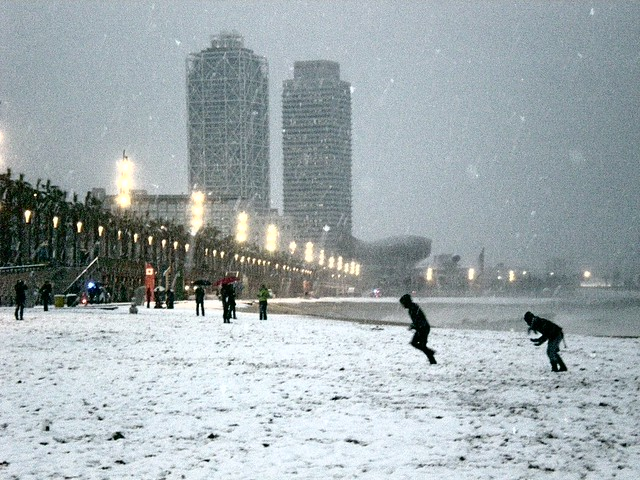
\includegraphics[height=1.2\paperheight]{vbreaks/vb2.jpg}
\end{frame}





\begin{frame}{Chapter 2: Functions of one variable}

A \textcolor{SeaGreen}{one-variable function} assigns a unique $y\in\mathbb{R}$ to each $x\in\mathbb{R}$: $y=f(x)$. 
\vskip 10pt
$x$: independent (exogenous) variable; $y$: dependent (endogenous) variable.
\vskip 8pt
\textcolor{SeaGreen}{Examples in econ/data:} cost, revenue, demand, utility, probability of purchase vs. price, click-through rate vs. ad spend, etc.
\vskip 8pt
\textcolor{SeaGreen}{Read} Ch. 3 Werner-Sotskov; Simon-Blume 2.1-2.2, 5.1-5.3.
\end{frame}

\begin{frame}{Graph and domain}

\begin{block}{Definition}
The \textcolor{SeaGreen}{graph} of $f$ is $\{(x,y)\in\mathbb{R}^2: y=f(x)\}$.
\vskip 6pt
The \textcolor{SeaGreen}{domain} $D$ is the set of $x$ where $f(x)$ is defined. \\[4pt]
\textcolor{SeaGreen}{Notation:} \hl{$f:D \rightarrow \mathbb{R}$}.	
\end{block}
\bigskip

\textcolor{SeaGreen}{Example}: $f(x)=\dfrac{1}{x}$ has $D=\mathbb{R}\setminus\{0\}$. 
\smallskip

Sometimes we restrict the domain (e.g., prices $x\ge 0$).
\end{frame}


\begin{frame}{Properties of functions}
A function $f:D \rightarrow \mathbb{R}$ is \textcolor{SeaGreen}{increasing} if 
$f(x_1)\le f(x_2)$ for any $x_1<x_2$ in $D$ (strict if $<$).\\[6pt]
\textcolor{SeaGreen}{Decreasing}: reverse inequality.\\[6pt]
\textcolor{SeaGreen}{Bounded}: $\exists C>0$ s.t. $|f(x)|\le C$ for all $x\in D$. 
\bigskip

\textcolor{SeaGreen}{Examples:}
\begin{itemize}
\item \textbf{Price-demand curve} often decreasing on realistic intervals.
\item \textbf{Learning curve} (error vs. epochs) typically decreasing and bounded below by $0$.
\end{itemize}
\end{frame}



\begin{frame}{Convex/concave functions}
For $x_1<x_2$ and $t\in[0,1]$, the \textcolor{SeaGreen}{convex combination} is $tx_1+(1-t)x_2$.\\[4pt]
A set $D\subset\mathbb{R}$ is \textcolor{SeaGreen}{convex} if it contains convex combinations.\\[6pt]
A function $f:D\to\mathbb{R}$ on convex $D$ is \textcolor{SeaGreen}{convex} if
\[
f(tx_1+(1-t)x_2)\le tf(x_1)+(1-t)f(x_2)
\]
(and \textcolor{SeaGreen}{concave} if $\ge$). Strict versions replace $\le$ by $<$ for $t\in(0,1)$ and $x_1\ne x_2$.
\end{frame}

\begin{frame}{Convex function}
\begin{figure}
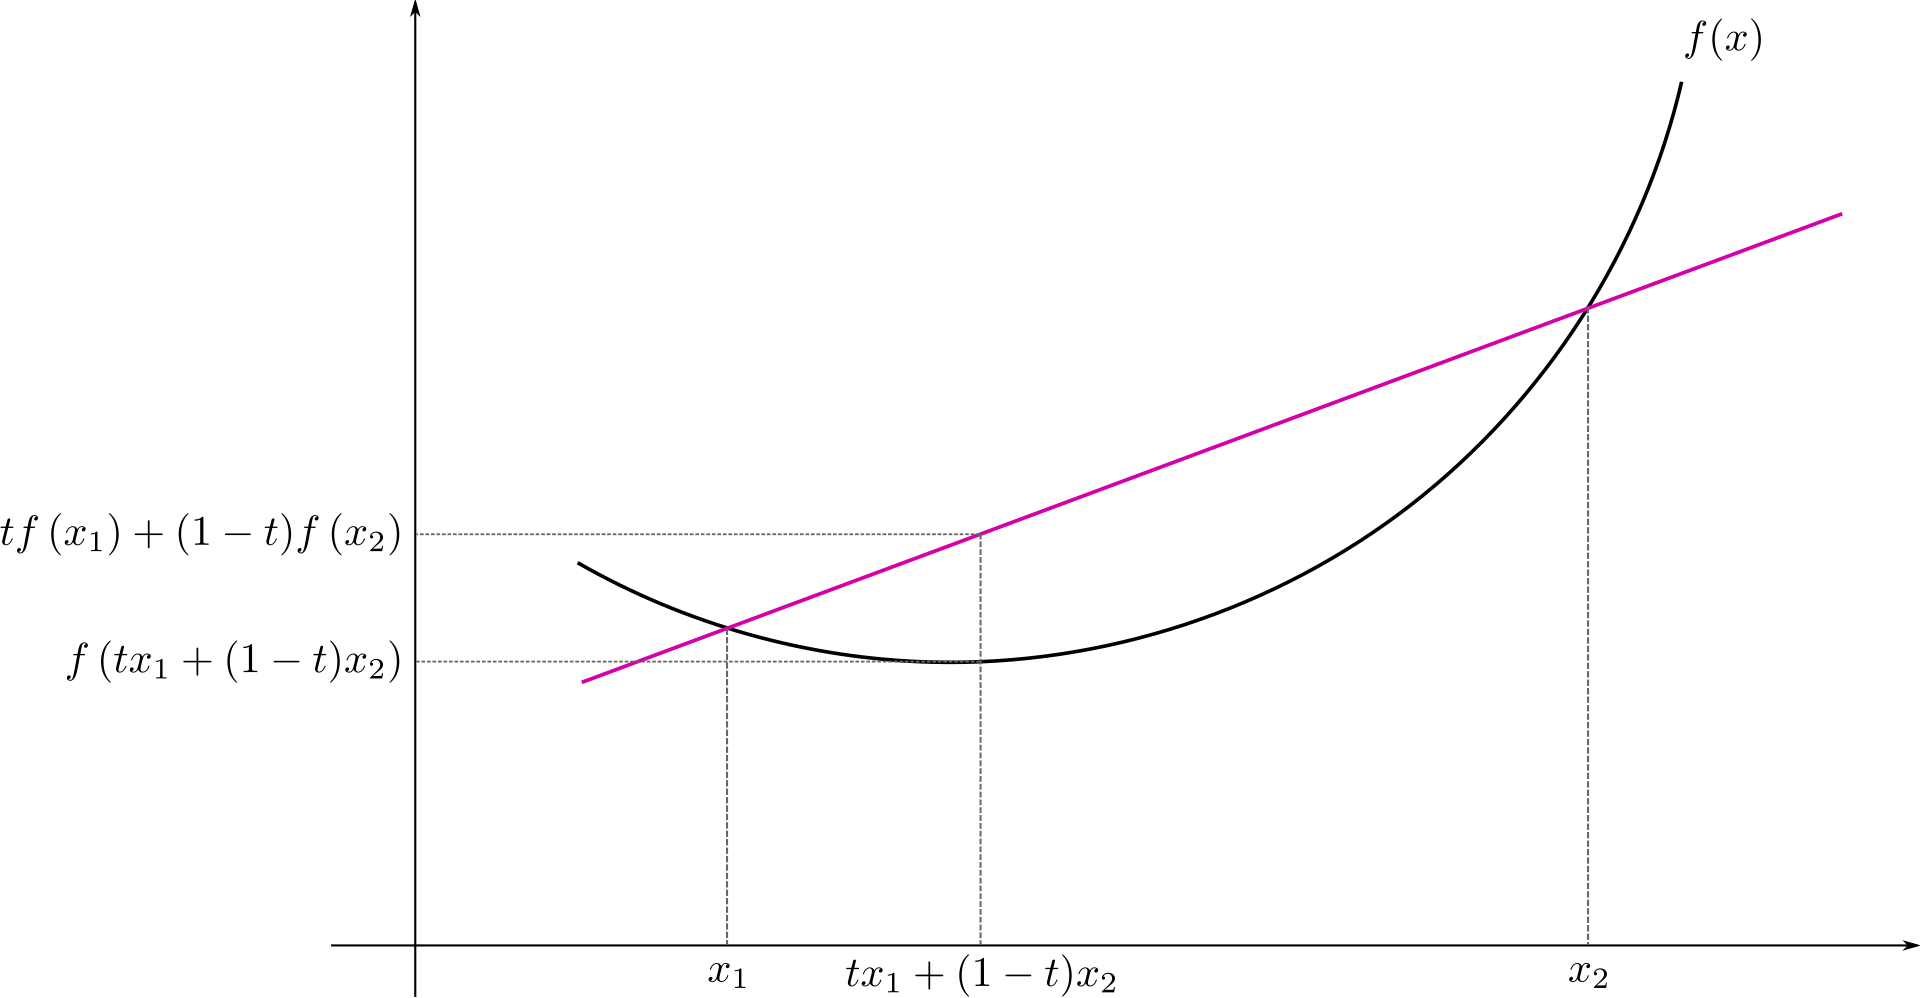
\includegraphics[width=4in]{img/convex} 
\end{figure}
\end{frame}



\begin{frame}{Quasi-convex/concave functions}
$f$ is \textcolor{SeaGreen}{quasi-convex} if
\[
f(tx_1+(1-t)x_2)\le \max\{f(x_1),f(x_2)\}.
\]
\textcolor{SeaGreen}{Quasi-concave} if $\ge \min\{f(x_1),f(x_2)\}$.
\bigskip

\textcolor{SeaGreen}{Facts:} convex $\Rightarrow$ quasi-convex; concave $\Rightarrow$ quasi-concave.\\[4mm]
Any \textcolor{SeaGreen}{strictly increasing} function is both quasi-convex and quasi-concave.\\[4mm]
\smallskip

\textcolor{SeaGreen}{Economic examples:} Indifference curves are typically quasi-convex; profit in price can be quasi-concave on feasible ranges.
\end{frame}

\begin{frame}{Economic example: logistic growth (adoption curves)}
The logistic function 
\[
f(t) = \frac{L}{1 + e^{-k(t - t_0)}}
\]
models \textcolor{SeaGreen}{technology/product adoption} or \textcolor{SeaGreen}{viral spread}. Early exponential growth, mid-phase inflection at $t_0$, saturation near $L$ (market size).
\begin{minipage}{6cm}{}
	\begin{figure}
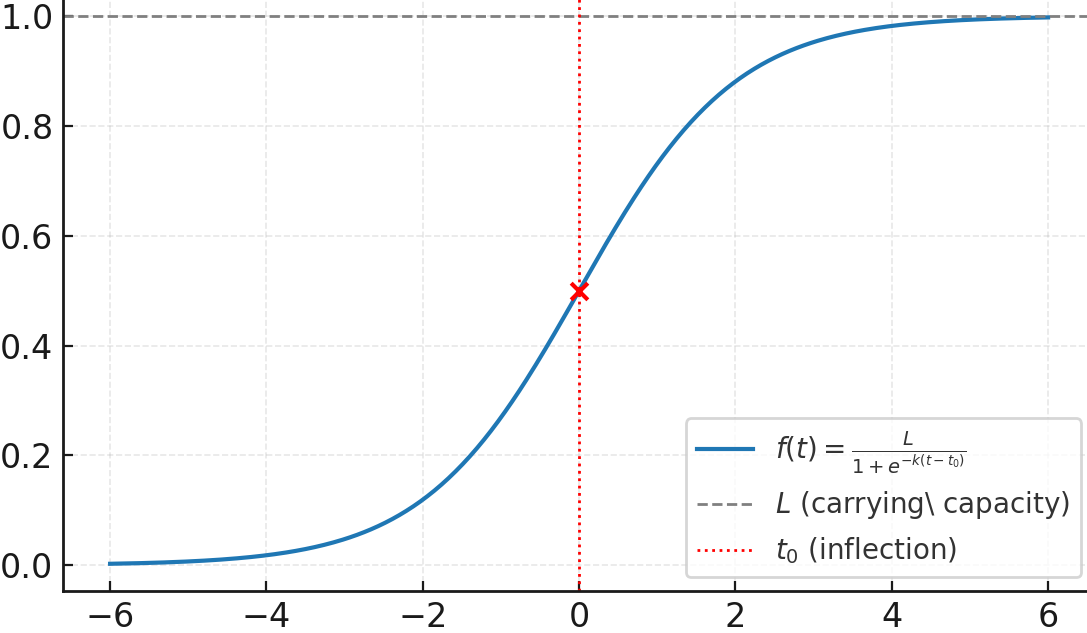
\includegraphics[width=2in]{img/returns1.png} 
\end{figure}
\end{minipage}\begin{minipage}{9cm}{}
\small
Interpretation: growth accelerates, then slows as saturation/frictions (capacity, regulation, budgets) bind. Same shape often appears in \textcolor{SeaGreen}{learning curves} (accuracy vs. data).
\end{minipage}
\end{frame}

\begin{frame}{Epidemics and beyond}

Logistic curves fit \textcolor{SeaGreen}{epidemic growth}, but also \textcolor{SeaGreen}{market penetration, platform adoption, content diffusion}. Check the following epidemic curves over time of the COVID-19 in China

\begin{figure}
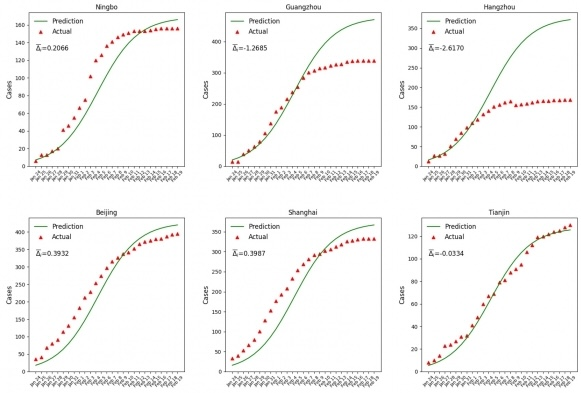
\includegraphics[width=0.60\textwidth]{img/figure}
\end{figure}
\end{frame}

\begin{frame}[plain]{}
\begin{tikzpicture}[remember picture,overlay]
  % Base image (centered; name it if you want to reference it later)
  \node[inner sep=0,anchor=center,yshift=-0.67\paperheight] (bg) at (current page.center)
       {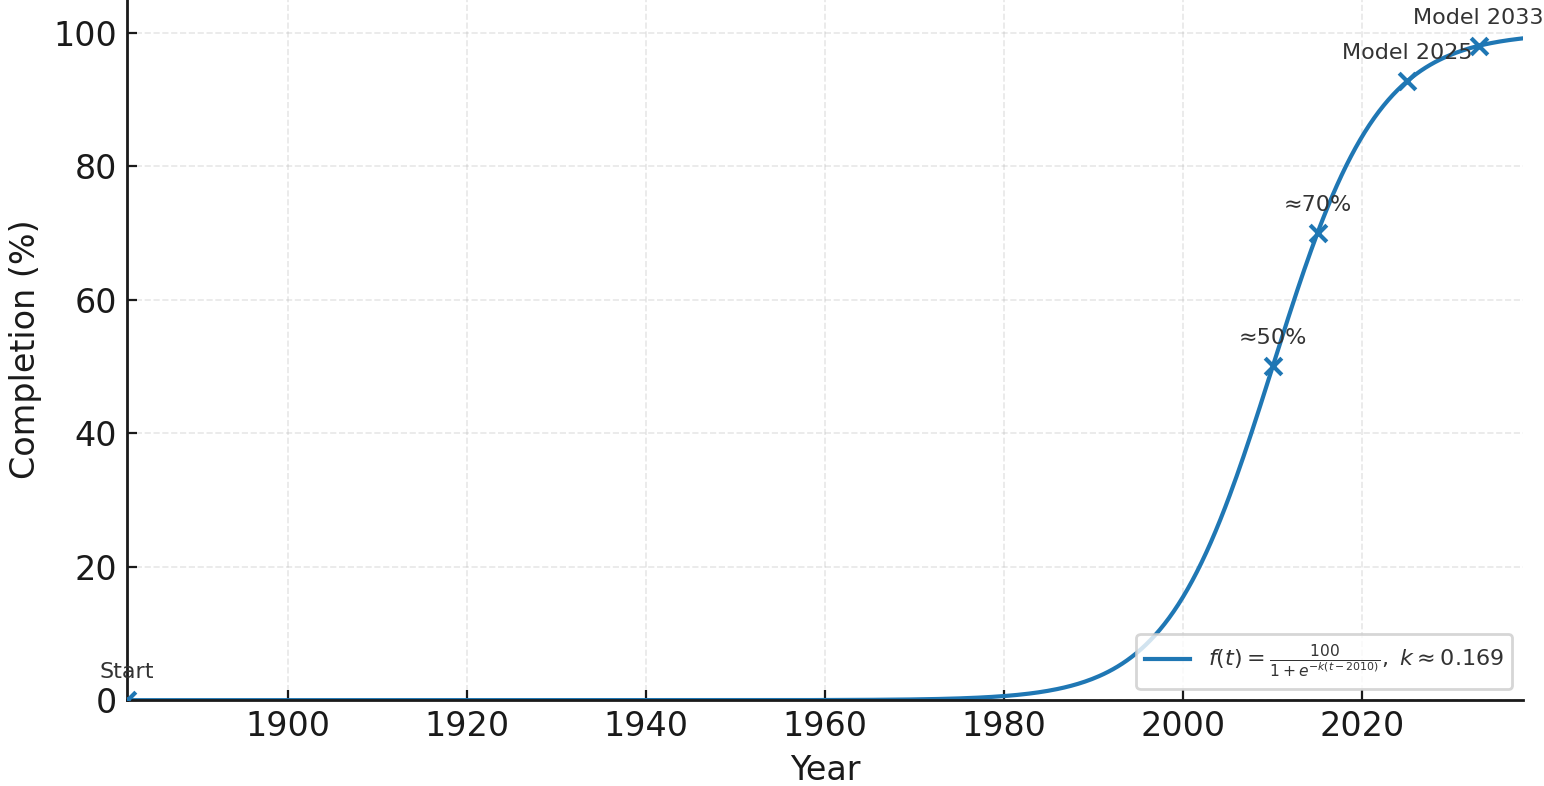
\includegraphics[scale=0.7]{img/SFprogress0.png}};

  % Overlay image: place relative to page, with fine offsets
 \only<2>{ \node[anchor=north west,
        xshift=0.2\paperwidth, % move right
        yshift=-0.8\paperheight] % move down
        at (current page.north west)
       {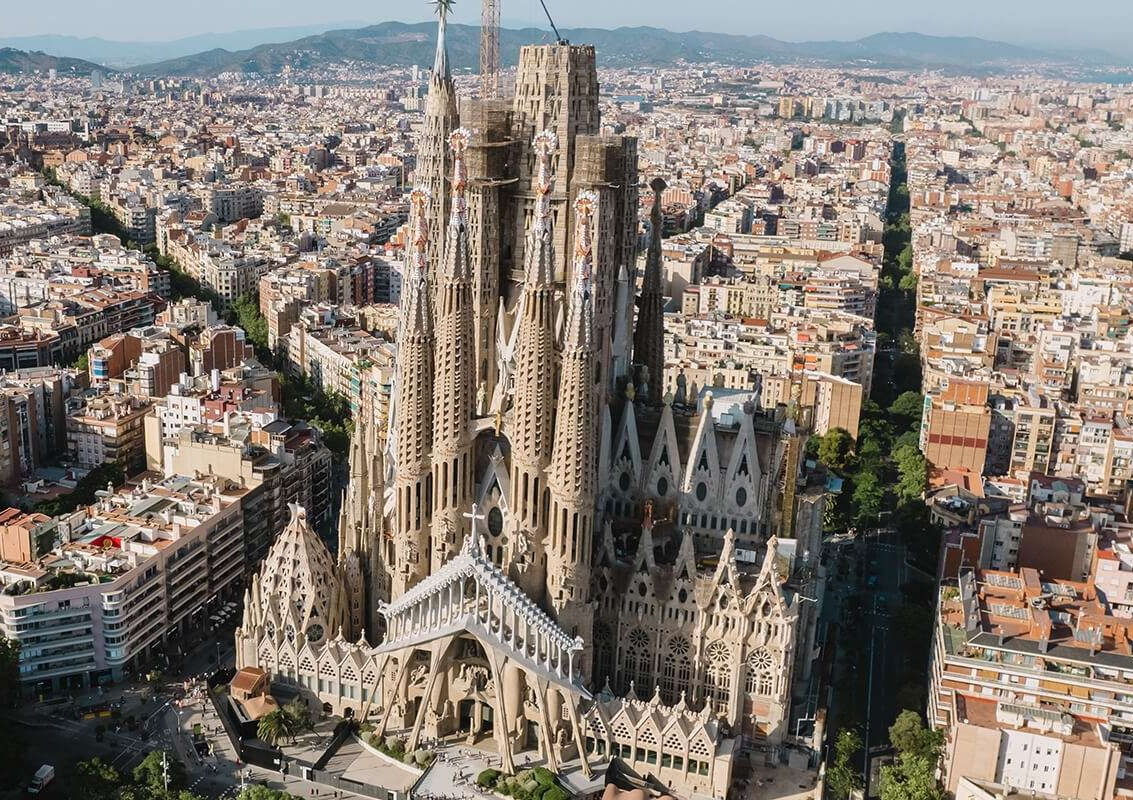
\includegraphics[width=0.45\paperwidth]{img/SF.jpg}};}
\end{tikzpicture}
\end{frame}

\begin{frame}{Examples of functions}

\begin{enumerate}
\item \textcolor{SeaGreen}{Monomials}: $f(x)=a x^k$
\item \textcolor{SeaGreen}{Polynomials}: sums of monomials
\item \textcolor{SeaGreen}{Rational}: ratios of polynomials
\item \textcolor{SeaGreen}{Exponential}: $f(x)=a^x$
\item \textcolor{SeaGreen}{Trig}: $\sin x$, $\cos x$, \ldots
\item \textcolor{SeaGreen}{Linear}: $f(x)=mx+b$ \begin{tiny}(slope $m$, intercept $b$; also $y-f(x_0)=m(x-x_0)$)\end{tiny}
\item \textcolor{SeaGreen}{Natural exponential}: $f(x)=e^x$ \begin{tiny}($e^x=\lim_n (1+\frac{x}{n})^n$)\end{tiny}
\item \textcolor{SeaGreen}{Natural log}: $f(x)=\log x$ \begin{tiny}($e^{\log x}=x$, $\log(e^x)=x$)\end{tiny}
\end{enumerate}

\smallskip
\textcolor{SeaGreen}{Econ view:} demand curves (often decreasing), cost curves (often convex), utility (often concave), isoelastic forms, log-sum-exp in discrete choice.
\end{frame}

\begin{frame}{Exponential functions}
\begin{figure}
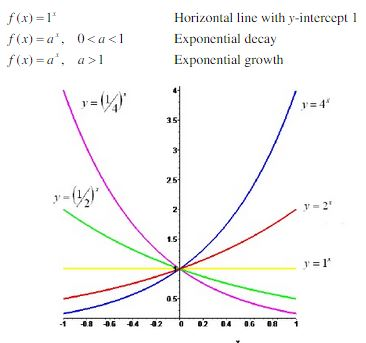
\includegraphics[width=2.5in]{img/exp} 
\end{figure}
\end{frame}

\begin{frame}{Chapter 3: Differentiation}

 \textcolor{SeaGreen}{Differentiation} measures sensitivity: how $f(x)$ changes with small changes in $x$.
\vskip 8pt
\textcolor{SeaGreen}{Examples:} price $\to$ demand sensitivity, ad spend $\to$ clicks, carbon tax $\to$ emissions, risk $\to$ portfolio value.\\[6pt]
Calculus also underpins extrema, monotonicity, convexity --- and the local behavior behind optimization and ML.
\vskip 6pt
\textcolor{SeaGreen}{Read} Ch. 4 Werner-Sotskov; Simon-Blume Chs. 2-5.
\vskip 12pt
\textcolor{SeaGreen}{Exercises:} 4.6(c), 4.10, 4.14, 4.15(a)-(c), 4.16(d), 4.17(b) (Werner-Sotskov), 5.5 (b)-(c)-(e) (Simon-Blume)

\end{frame}


\begin{frame}{Limit of a function}
\begin{alertblock}{}
Let $f:D  \rightarrow \mathbb{R}$ and $x_0 \in \mathbb{R}$. $L=\lim_{x\to x_0} f(x)$ if for any sequence $x_n\in D$ with $x_n\to x_0$, we have $f(x_n)\to L$. 	\\[2mm]
\textcolor{SeaGreen}{Remark:} $x_0$ need not be in $D$ (removable/essential discontinuities matter in econ too).
\end{alertblock}
 \textcolor{SeaGreen}{Example:} $\lim_{x \rightarrow 0} x \sin\frac{1}{x}=0$ since $0\leq | x \sin\frac{1}{x}| \leq |x|$.
\begin{block}{Algebra of limits}
If $\lim f = y_1$ and $\lim g = y_2$ at $x_0$, then
\[
\lim (f+g)=y_1+y_2,\quad 
\lim (fg)=y_1 y_2,\quad 
\lim \frac{f}{g}=\frac{y_1}{y_2}\text{ if }y_2\ne 0,\,g\ne 0\text{ near }x_0.
\]
\end{block}
\end{frame}

\begin{frame}{Continuity}

\begin{alertblock}{Definition}
$f$ is \textcolor{SeaGreen}{continuous} at $x_0\in D$ if $\lim_{x\to x_0} f(x)=f(x_0)$.
If $f$ is continuous at every point of $B\subset D$, we say $f$ is continuous on $B$.	
\end{alertblock}
\bigskip 


\textcolor{SeaGreen}{Theorem:} If $f,g$ are continuous at $x_0$ then so are $f+g$ and $f g$. If moreover,
$g(x)\neq 0$ around $x_0$, then $\frac{f}{g}$ is continuous at $x_0$.

\vskip 8pt
\textcolor{SeaGreen}{Heine-Borel fact (1D):} continuous $f:[a,b]\to\mathbb{R}$ is bounded.
\end{frame}


\begin{frame}{Composition and inverse}
\begin{alertblock}{Two important results}
(composition) If $f,g$ are continuous, so is $h=g\circ f$; moreover
\[
\lim_{x\to x_0} g(f(x))=g\!\left(\lim_{x\to x_0}f(x)\right).
\]
(inverse)	If $f:[a,b]\to\mathbb{R}$ is strictly monotone and continuous with $f(a)=c,f(b)=d$, then the inverse $f^{-1}:[c,d]\to[a,b]$ is also strictly monotone and continuous.
\end{alertblock}
\textcolor{SeaGreen}{Econ:}  
Let \( p \) denote the price of a good and \( q \) the quantity sold.  
The \emph{demand function} \( q(p) \) gives the quantity \( q \) consumers will buy at price \( p \).  
Equivalently, the \emph{inverse demand function} \( p(q) \) gives the price at which \( q \) units can be sold.  Revenue as a function of quantity is:
\[
R(q) = p(q) \cdot q,
\]
which involves compositions.
\end{frame}

\begin{frame}{Derivative}

Let $f:(a,b) \rightarrow \mathbb{R}$. $f$ is \textcolor{SeaGreen}{differentiable} at $x$ if
\[
\lim_{h \rightarrow 0} \frac{f(x+h)-f(x)}{h}
\]
exists. Denote this limit by \hl{$f'(x)$}.\\[4mm]

\textcolor{SeaGreen}{Fact:} differentiable $\Rightarrow$ continuous (not conversely: $|x|$ is continuous but not differentiable at $0$).\\[4mm]

\textcolor{SeaGreen}{Interpretation:} local linear approximation --- crucial in marginal analysis, price elasticity, and gradient-based optimization.
\end{frame}

\begin{frame}{Geometric interpretation}
If $f$ is differentiable at $x_0$, the tangent line at $(x_0,f(x_0))$ is
\[
y=f(x_0)+f'(x_0)(x-x_0).
\]
\begin{figure}
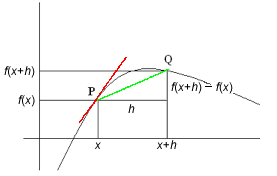
\includegraphics[width=2.5in]{img/derivative} \\
\small slope of \textcolor{green}{secant} through P,Q: $\frac{f(x+h)-f(x)}{h}$;\quad
slope of \textcolor{red}{tangent} at P: $f'(x)$
\end{figure}
\end{frame}


\begin{frame}{A ``marginal'' is a derivative}
In economics, a \textbf{marginal} quantity measures how much something changes when we increase an input by a small amount. Mathematically, we often approximate
\[
f(x+1) - f(x)\;\approx\;f'(x) ,
\]
when the change is 1 unit.\\[3mm]

\textcolor{SeaGreen}{Examples:}
\begin{itemize}
\item \textbf{Marginal revenue:} $\frac{d}{dq}[p(q)\,q]$ at the current sales level $q$.  
The derivative tells you how much extra revenue you gain (or lose) by selling one more unit.
\item \textbf{Click-through sensitivity:} $\frac{d\,\text{CTR}}{d(\text{ad spend})}$ at the budget currently in use.  
Here CTR (click-through rate) is a function of ad spending; the derivative measures how much CTR improves with an extra euro of spending.\\[4mm]
%\item \textbf{Emissions response:} $\frac{dE}{d\tau}$ with respect to a carbon tax $\tau$.  
%This shows how a small increase in the carbon tax changes total emissions $E$.
\end{itemize}

If the change is $\Delta x$ rather than $1$:\quad  $f(x+\Delta x)-f(x)\approx f'(x)\,\Delta x $.\\[3mm]
In differential notation: \quad\quad\quad\quad\quad $df \approx f'(x)\,dx$
\end{frame}



\begin{frame}{Derivatives of elementary functions}
\begin{enumerate}
\item $c' =0$
\item $(x^n)'=nx^{n-1}$ for $n\in\mathbb{N}$
\item $(x^\alpha)'=\alpha x^{\alpha-1}$ for $\alpha\in\mathbb{R}$, $x>0$
\item $(\log x)'=\dfrac{1}{x}$, $x>0$
\item $(\sin x)'=\cos x$
\item $(\cos x)'=-\sin x$
\item $(e^x)'=e^x$
\item $(a^x)'=a^x\log a$, $a>0$
\end{enumerate}
\begin{tiny}Proof of 8: $(a^x)'=(e^{x\log a})'=a^x\log a$ (chain rule)\end{tiny}
\end{frame}

\begin{frame}{Product/quotient rules}
If $f,g$ are differentiable:
\begin{itemize}
\item $(f+g)'=f'+g'$\\[4mm]
\item $(fg)'=f'g+g'f$ \quad \text{[Leibniz rule]}\\[4mm]
\item $\left(\dfrac{f}{g}\right)'=\dfrac{f'g-g'f}{g^2}$ where $g\ne 0$ near the point.\\[7mm]
\end{itemize}
\smallskip
\textcolor{SeaGreen}{Example (revenue):} $R(q)=p(q)\,q$, then $R'(q)=p'(q)\,q+p(q)$.
\end{frame}

\begin{frame}{Chain rule}
\begin{alertblock}{}
If $h=g\circ f$ and $f,g$ are differentiable at the relevant points, then
\[
h'(x)=g'(f(x))\,f'(x).
\]
\end{alertblock}

\textcolor{SeaGreen}{Example (cost of production):}
\[
C(x)=4+\log(x+1)+\sqrt{3x+1}\quad\Rightarrow\quad
C'(x)=\frac{1}{x+1}+\frac{3}{2\sqrt{3x+1}}.
\]
\textcolor{SeaGreen}{Example (choice models):} In discrete choice models, the logistic function 
$\sigma(x)=\tfrac{1}{1+e^{-x}}$ maps a score $x$ (reflecting how attractive an option is) 
to the probability of choosing it. Its derivative $\sigma'(x)=\sigma(x)[1-\sigma(x)]$ 
measures how sensitive the choice probability is to changes in $x$.\end{frame}




\begin{frame}{Differentiating $u(x)^{v(x)}$}
\small
Let $u(x) > 0$. For $h(x) = u(x)^{v(x)}$, taking logs gives:
\[
\log h = v\log u
\quad\Rightarrow\quad
\frac{h'}{h} = v'\log u + v\,\frac{u'}{u}.
\]
Hence
\[
\boxed{\;h'(x) = u(x)^{v(x)}\Big(v'(x)\log u(x) + v(x)\,\frac{u'(x)}{u(x)}\Big)\;}
\]

\medskip
\textcolor{SeaGreen}{Econ example:}  
A startup's valuation is $V(t) = V_0[1+g(t)]^{T(t)}$, where  
$g(t)$ is the projected annual growth rate and $T(t)$ the number of years that growth lasts.  
Both $g(t)$ and $T(t)$ vary with $t$.
\end{frame}

\begin{frame}{Some of the contributors (in form of \textit{caganers})}
	\centering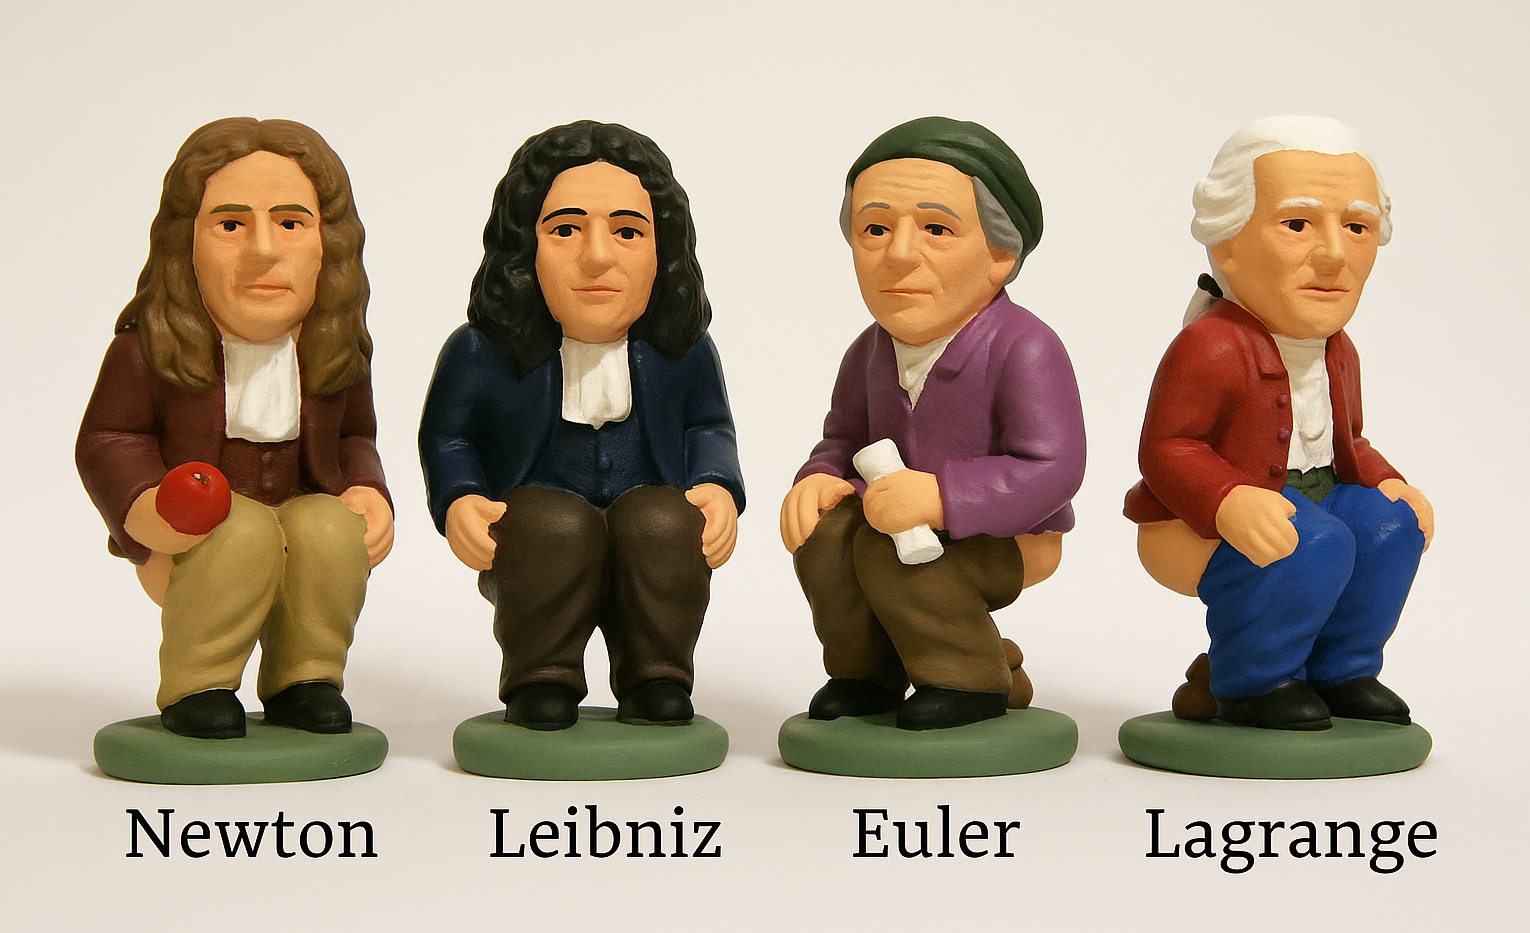
\includegraphics[scale=.25]{vbreaks/caganer1}
\end{frame}

\begin{frame}{Derivative of the inverse}

\textcolor{SeaGreen}{Theorem:} If $f$ is strictly monotone, continuous, and differentiable at $x$ with $f'(x)\ne 0$, then $f^{-1}$ is differentiable at $y=f(x)$ and
\[
(f^{-1})'(y)=\frac{1}{f'(x)}=\frac{1}{f'(f^{-1}(y))}.
\]
\begin{tiny}Since $f^{-1}(f(x))=x$, chain rule gives $(f^{-1})'(f(x))f'(x)=1$.\end{tiny}
\bigskip

\textcolor{SeaGreen}{Example:} $f(x)=e^x$ $\Rightarrow$ $(\log)'(y)=1/y$.
\bigskip

\textcolor{SeaGreen}{Higher-order derivatives:} If $f'$ is differentiable,  its derivative is called the \textcolor{SeaGreen}{second derivative} of $f$ and  denoted $f''$. Similarly, we can define \textcolor{SeaGreen}{higher-order derivatives}, and $f^{(n)}$ is called the $n$th derivative of $f$. If $f^{(n)}$ is continuous, we say that $f$ is $n$ times \textcolor{SeaGreen}{continuously differentiable} or \hl{$C^{n}$} for short.
\end{frame}

\begin{frame}{L'H\^opital's rule}

 \textcolor{SeaGreen}{Theorem:} Let $f,g$ be $C^1$ on $(a,b)$ with $g'\ne 0$ on $(a,b)$. If
\[
\lim_{x\to x_0} f(x)=\lim_{x\to x_0} g(x)=0\quad\text{or}\quad \pm\infty,
\]
then
\[
\lim_{x\to x_0}\frac{f(x)}{g(x)}=\lim_{x\to x_0}\frac{f'(x)}{g'(x)} \quad\text{(if the RHS limit exists)}.
\]
\begin{tiny}Proof idea uses the Mean Value Theorem (slide~\ref{mv}).\end{tiny}
\bigskip

\textcolor{SeaGreen}{Example:} 
\[
\lim_{x\to 0}(1+x)^{1/x}
= \exp\!\left(\lim_{x\to 0}\frac{\log(1+x)}{x}\right)
= \exp\!\left(\lim_{x\to 0}\frac{1}{1+x}\right)=e.
\]
\end{frame}

\begin{frame}{Monotonicity via derivatives}

If $f$ is differentiable on $(a,b)$:
\begin{enumerate}
\item $f$ increasing on $[a,b]$ $\Longleftrightarrow$ $f'(x)\ge 0$ on $(a,b)$.
\item $f$ decreasing on $[a,b]$ $\Longleftrightarrow$ $f'(x)\le 0$ on $(a,b)$.
\item $f$ constant on $[a,b]$ $\Longleftrightarrow$ $f'(x)=0$ on $(a,b)$.
\item $f'(x)>0$ on $(a,b)$ $\Rightarrow$ $f$ strictly increasing on $[a,b]$.
\item $f'(x)<0$ on $(a,b)$ $\Rightarrow$ $f$ strictly decreasing on $[a,b]$.
\end{enumerate}
\begin{tiny}Converse of 4-5 can fail at isolated points (e.g., $x^3$).\end{tiny}
\bigskip

\textcolor{SeaGreen}{Example:} $f(x)=\frac{x^3}{3}+2x^2+3x+1$; $f'(x)=(x+1)(x+3)$ determines monotonicity intervals and local extrema.
\end{frame}

\begin{frame}{Optimal points: first-order conditions}
\begin{block}{Local optima}
Let $f:D\to\mathbb{R}$. A point $x_0\in D$ is a \textcolor{SeaGreen}{local max} if $\exists (a,b)\subset D$ with $x_0\in(a,b)$ and $f(x)\le f(x_0)$ for all $x\in(a,b)$.
Similarly for \textcolor{SeaGreen}{local min} with $\ge$.\\[4mm]
	
\end{block}

\smallskip

If $f$ has a local optimum at interior $x$ and is differentiable, then $f'(x)=0$ (\textcolor{SeaGreen}{necessary}, not sufficient).\\[4mm]
\smallskip

\textcolor{SeaGreen}{Economic flavor:} 
In profit maximization, the optimal quantity $q^*$ often satisfies the first-order condition $f'(q^*)=0$,  
which, for profit $\pi(q) = R(q) - C(q)$, means \emph{marginal revenue} $R'(q)$ equals \emph{marginal cost} $C'(q)$.\\[4mm]

If $x$ is stationary ($f'(x)=0$) and $f$ is strictly increasing to the left and strictly decreasing to the right, then $x$ is a local max (reverse for min).

\end{frame}

\begin{frame}{Optimal points}
\begin{figure}
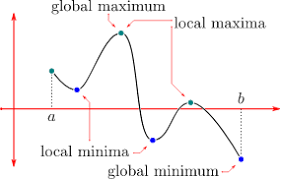
\includegraphics[width=2.5in]{img/max_min} 
\end{figure}
\end{frame}


\begin{frame}{Example: Timing a sale (present value)}

Suppose an asset’s market value is $V(t)$ at time $t$.  
At a constant annual interest rate $R$, the \textbf{present value} of selling at time $t$ is
\[
P(t) = V(t)\,e^{-Rt},
\]
where $e^{-Rt}$ discounts future cash flows.

\smallskip
\textcolor{SeaGreen}{Goal:} Choose $t$ to maximize $P(t)$.

\smallskip
\textcolor{SeaGreen}{FOC (set derivative to zero):}
\[
P'(t) = V'(t)e^{-Rt} - R\,V(t)e^{-Rt} = 0
\quad\Rightarrow\quad \frac{V'(t)}{V(t)} = R.
\]

\textcolor{SeaGreen}{Interpretation:} Sell when the asset’s \emph{instantaneous percentage growth rate}  
(matches) the \emph{interest rate you could earn in the bank}.

\bigskip
\textcolor{SeaGreen}{Example:} If $V(t) = 10000\,e^{\sqrt{t}}$ and $R = 6\%$,  
then $P(t) = 10000\,e^{\sqrt{t} - 0.06\,t}$, which is maximized near $t \approx 69.44$.
\end{frame}
\begin{frame}{Plot of the present value $P(t)$}
\begin{figure}
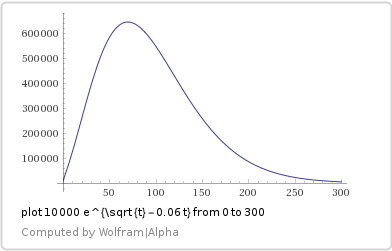
\includegraphics[width=3.5in]{img/plot} 
\end{figure}
To certify a \textcolor{SeaGreen}{global} optimum on an interval, compare values at boundaries and critical points. Here $P(0)=10000$, $\lim_{t\to\infty}P(t)=0$.
\end{frame}

\begin{frame}{Second-order conditions}

\textcolor{SeaGreen}{Test:} If $f'(x_*)=0$ and $f''(x_*)<0$ ($>0$), then $x_*$ is a strict local max (min). Higher-order tests extend this when $f''(x_*)=0$.
\smallskip

\textcolor{SeaGreen}{Example:} For $f(x)=\dfrac{\log^2(3x)}{x}$ ($x>0$): 
\[
f'(x)=\frac{(2-\log 3x)\log 3x}{x^2},\quad
f''(x)=\frac{2(1-3\log 3x + \log^2 3x)}{x^3}.
\]
Critical points at $x_1=\frac{1}{3}$ (min), $x_2=\frac{e^2}{3}$ (max).
\end{frame}


\begin{frame}{Plot of $f(x)=\dfrac{\log^2 3x}{x}$, $x>0$}

\begin{figure}
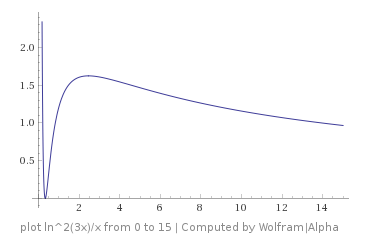
\includegraphics[width=3.5in]{img/ima} 
\end{figure}
$\lim_{x \rightarrow \infty} f(x)=0$, $\lim_{x \rightarrow 0^+} f(x)=\infty$,
$f(x_1)=0$, $f(x_2)>0$ $\Rightarrow$ $x_1$ global min, no global max.
\end{frame}



\begin{frame}{Convexity and concavity}

If $f$ is twice differentiable on $(a,b)$:
\begin{enumerate}
\item $f$ convex on $[a,b]$ $\Leftrightarrow$ $f''(x)\ge 0$ for all $x\in(a,b)$.
\item $f$ concave on $[a,b]$ $\Leftrightarrow$ $f''(x)\le 0$ for all $x\in(a,b)$.
\item $f''>0$ ($<0$) $\Rightarrow$ $f$ strictly convex (concave).
\end{enumerate}
\bigskip

 \textcolor{SeaGreen}{Theorem:} If $f$ and $g$ are convex (or concave), then $f \circ g$ is convex (or concave).
 
\textcolor{SeaGreen}{Example:} $f(x)=e^{x^2}$ is strictly convex on $[0, \infty)$.

\bigskip

\textcolor{SeaGreen}{Economics:} costs often convex; utility often concave; regularized losses in ML are designed to be convex for tractable optimization.
\end{frame}

\begin{frame}{Example of changing curvature}

Let $f(x)=\dfrac{2x}{x^2+1}$. Then
\[
f'(x)=\frac{2(1-x^2)}{(x^2+1)^2},\qquad 
f''(x)=\frac{4(x^3-3x)}{(x^2+1)^3}.
\]
So $f$ is strictly convex on $[-\sqrt{3},0]\cup [\sqrt{3},\infty)$ and strictly concave on $(-\infty,-\sqrt{3}]\cup[0,\sqrt{3}]$.
\end{frame}

\begin{frame}{Plot of $f(x)=\dfrac{2x}{x^2+1}$}

\begin{figure}
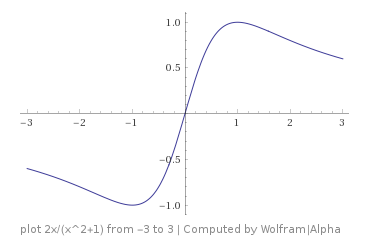
\includegraphics[width=3.5in]{img/ima1} 
\end{figure}

Inflexion points at $x\in\{-\sqrt{3},0,\sqrt{3}\}$. Global max at $x=1$, min at $x=-1$, and $\lim_{|x|\to\infty} f(x)=0$.
\end{frame}

\begin{frame}{Inflexion points}
If $f$ is $C^n$ on $(a,b)$, an \textcolor{SeaGreen}{inflexion point} at $x_*$ occurs when curvature changes sign. A sufficient test: 
\[
f''(x_*)=\cdots=f^{(n-1)}(x_*)=0,\quad f^{(n)}(x_*)\ne 0,\quad n\ \text{odd}.
\]
\textcolor{SeaGreen}{Example:} $f(x)=x^3$ has $f''(0)=0$, $f^{(3)}(0)=6\ne 0$ $\Rightarrow$ inflexion at $0$.
\end{frame}


\begin{frame}[label=mv]{Mean-value theorem}
\begin{alertblock}{Mean Value Theorem}
If $f$ is continuous on $[a,b]$ and differentiable on $(a,b)$,
then $\exists c\in(a,b)$ such that
\[
f'(c)=\frac{f(b)-f(a)}{b-a}\quad(\text{equivalently } f(b)=f(a)+f'(c)(b-a)).
\]
\end{alertblock}
\begin{tiny}Proof idea: consider $h(x)=(f(b)-f(a))x-(b-a)f(x)$; since $h(a)=h(b)$, $h$ has an interior extremum.\end{tiny}
\bigskip

\textcolor{SeaGreen}{Interpretation:} the instantaneous slope matches the secant slope at some point.
\end{frame}

\begin{frame}{Geometry of the mean-value theorem}
Recall: $\exists c\in(a,b)$ s.t. 
\[
f'(c)=\frac{f(b)-f(a)}{b-a}.
\]
\begin{figure}
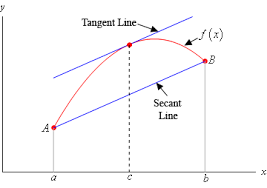
\includegraphics[width=2.5in]{img/secant} 
\end{figure}
\end{frame}

\begin{frame}{Taylor formula}
\textcolor{SeaGreen}{Theorem (Taylor's formula of order $n$):} Let $f$ be $n+1$ times differentiable on $(a,b)$,
 and let $x_0 \in (a,b)$ given. Then, for any $x \in (a,b)$,
 if $n=1$,
$$ f(x)=f(x_0)+f'(x_0)(x-x_0)+\text{error}.$$
%If  $n=2$
%$$f(x)=f(x_0)+f'(x_0)(x-x_0)+\frac{f''(x_0)}{2!}(x-x_0)^2+\text{error}.$$
If  $n\geq 2$,
 \begin{equation*} \begin{split}
 f(x)=\textcolor{DarkRed}{f(x_0)+f'(x_0)(x-x_0)+\frac{f''(x_0)}{2!}(x-x_0)^2+
\frac{f^{(n)}(x_0)}{n!}(x-x_0)^n}+\text{error}.
 \end{split}
 \end{equation*}
 
 
  The error is small if $x$ is close to $x_0$, therefore, this theorem says that differentiable functions may be \textcolor{SeaGreen}{locally approximated
 by a polynomial} called the \textcolor{DarkRed}{Taylor polynomial}.
 \bigskip

\textcolor{SeaGreen}{Economics/data:} local linear/quadratic approximations underlie elasticity (log-linearization), Delta method, and second-order price responses.
\end{frame}

\begin{frame}{Taylor remainder and a handy expansion}
\begin{alertblock}{Remainder (Lagrange form)}
\[
R_n^y(x)=\frac{f^{(n+1)}(y)}{(n+1)!}(x-x_0)^{n+1}\quad\text{for some }y\text{ between }x_0\text{ and }x.
\]
\end{alertblock}
If $|f^{(n+1)}|\le M$ near $x_0$, then $|R_n^y(x)|\le \dfrac{M}{(n+1)!}|x-x_0|^{n+1}$.
\smallskip

\textcolor{SeaGreen}{Example (log around 1):} With $x_0=1$,
\[
\log x \approx (x-1)-\tfrac12(x-1)^2,\quad 
R_2^y(x)=\frac{1}{3y^3}(x-1)^3.
\]
\textcolor{SeaGreen}{Finance quick check:} For small $r$, $\log(1+r)\approx r-\frac{r^2}{2}$ $\Rightarrow$ EAR $\approx$ APR $-\ \frac12 \text{APR}^2$ (small correction).
\end{frame}

% (Optional advanced finance slides removed as requested earlier; calculus focus retained.)


\begin{frame}{Short comment about small-o notation}
	Writing $|R_n^y(x)|\le \dfrac{M}{(n+1)!}|x-x_0|^{n+1}$ we conclude $\tfrac{R^y_n(x)}{|x-x_0|^{n}}\leq \dfrac{M}{(n+1)!}|x-x_0|$ and so
	$$
	\lim_{x\to x_0} \frac{R^y_n(x)}{|x-x_0|^{n}}\;=\;0.
	$$
	This we write as $ R^y_n(x)=o(|x-x_0|^{n})$.\\[5mm]
	
\begin{alertblock}{In particular: If $f$ is twice differentiable:}
	$f(x+h)\;=\;f(x)+f'(x)h + o(|h|)$.
\end{alertblock}
The generalization of this last expression to multivariate functions will provide powerful insights into their optimization. 
\end{frame}


\end{document}